\documentclass[aspectratio=169]{beamer}

\usetheme[progressbar=frametitle]{metropolis}
\usepackage{appendixnumberbeamer}

\usepackage{booktabs}
\usepackage[scale=2]{ccicons}

\usepackage{pgfplots}
\usepgfplotslibrary{dateplot}

\usepackage{hyperref}

\usepackage{pgfpages}

\usepackage{soul}

\usepackage{xspace}
\newcommand{\themename}{\textbf{\textsc{metropolis}}\xspace}

\usepackage[brazil]{babel}

\usepackage[outputdir=..]{minted}
		   
\newminted{verilog}{fontsize=\scriptsize, 
		   linenos,
		   breaklines,
		   numbersep=8pt,
           tabsize=2,
		   framesep=3mm} 
		   
\usepackage{multicol}
\usepackage{multirow}
\usepackage{subcaption}

\usepackage{graphicx}
\graphicspath{{figs/}}
\usepackage{graphbox}

\usepackage{pgf,tikz}
\usetikzlibrary{shapes,arrows,positioning}
\usetikzlibrary{circuits.logic.US}
\usetikzlibrary{matrix,calc}

\title{$\mu$P1}

\author{\large Prof. Ricardo Menotti (\href{mailto:menotti@ufscar.br}{menotti@ufscar.br})}

\date{Atualizado em: \today}

\institute{\large \textbf{Departamento de Computação} \\
Centro de Ciências Exatas e de Tecnologia \\
Universidade Federal de São Carlos}

\titlegraphic{\hfill\includegraphics[height=1.5cm]{LogoUfscar}}

\subtitle{Um processador simples} 

\begin{document}

\begin{frame}
	\titlepage
\end{frame} 

\begin{frame}{Processador - $\mu$P1 (8 bits) \cite{hamblen}} \centering
    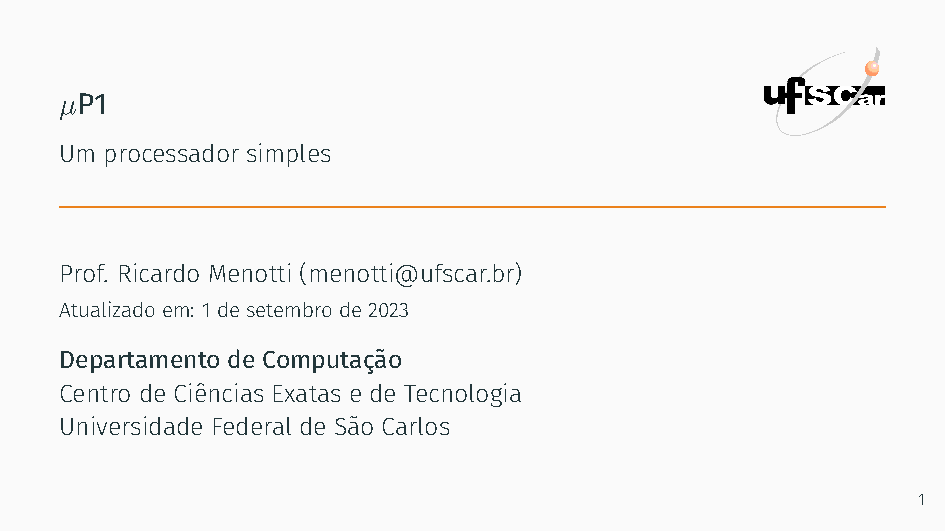
\includegraphics[width=\textwidth]{uP1}
\end{frame}

\begin{frame}{Organização de memória do $\mu$P1}
    \begin{multicols}{2}
    \begin{itemize}
        \item Instruções
    \end{itemize}    
    \begin{tabular}{ccccccccl}
        \hline
         \multicolumn{8}{c}{endereço} & \textit{palavras} \\
         \hline
         \hline
        0 & 0 & 0 & 0 & 0 & 0 & 0 & 0 & \multirow{5}{*}{$2^{7} = 128$} \\
        % \hline
        \multicolumn{8}{c}{.} \\
        \multicolumn{8}{c}{.} \\
        \multicolumn{8}{c}{.} \\
        % \hline
        0 & 1 & 1 & 1 & 1 & 1 & 1 & 1 &  \\
        \hline
    \end{tabular}
    \vfill\null
    \columnbreak
    \begin{itemize}
        \item Não alocada (N/A)
    \end{itemize}    
    \begin{tabular}{ccccccccl}
        \hline
         \multicolumn{8}{c}{endereço} & \textit{palavras} \\
         \hline
         \hline
        1 & 0 & 0 & 0 & 0 & 0 & 0 & 0 & \multirow{3}{*}{$2^{7} - 2^{4} = 112$} \\
        % \hline
        \multicolumn{8}{c}{.} \\
        % \hline
        1 & 1 & 1 & 0 & 1 & 1 & 1 & 1 &  \\
        \hline
    \end{tabular}
    \begin{itemize}
        \item Dados
    \end{itemize}    
    \begin{tabular}{ccccccccl}
        \hline
         \multicolumn{8}{c}{endereço} & \textit{palavras} \\
         \hline
         \hline
        1 & 1 & 1 & 1 & 0 & 0 & 0 & 0 & \multirow{3}{*}{$2^{4} = 16$} \\
        % \hline
        \multicolumn{8}{c}{.} \\
        % \hline
        1 & 1 & 1 & 1 & 1 & 1 & 1 & 1 &  \\
        \hline
    \end{tabular}    \end{multicols}
\end{frame}

\begin{frame}{Conjunto de instruções (ISA) do $\mu$P1 - 8 bits - 4 instruções - 2 formatos}
    \begin{multicols}{2}
        \textbf{Formato M} \\
        \texttt{Endereço: 0x1111\_endereço\_D}
    \begin{tabular}{|c|c|c|c|c|c|c|c|l|}
        \hline
         7 & 6 & 5 & 4 & 3 & 2 & 1 & 0 & \textit{bits} \\
         \hline
         \hline
        0 & 0 & 0 & 0 & \multicolumn{4}{c|}{endereço D} & \textit{N/A} \\
        % \hline
        0 & 0 & 0 & 1 & \multicolumn{4}{c|}{endereço D} & \textit{N/A} \\
        % \hline
        0 & 0 & 1 & 0 & \multicolumn{4}{c|}{endereço D} & \textit{N/A} \\
        % \hline
        0 & 0 & 1 & 1 & \multicolumn{4}{c|}{endereço D} & STORE \\
        % \hline
        0 & 1 & 0 & 0 & \multicolumn{4}{c|}{endereço D} & LOAD \\
        % \hline
        0 & 1 & 0 & 1 & \multicolumn{4}{c|}{endereço D} & ADD  \\
        % \hline
        0 & 1 & 1 & 0 & \multicolumn{4}{c|}{endereço D} & \textit{N/A} \\
        % \hline
        0 & 1 & 1 & 1 & \multicolumn{4}{c|}{endereço D} & \textit{N/A} \\
        \hline
    \end{tabular}
        \textbf{Formato J} \\
        \texttt{Endereço: 0x0\_endereço\_I}
    \begin{tabular}{|c|c|c|c|c|c|c|c|l|}
        \hline
        7 & 6 & 5 & 4 & 3 & 2 & 1 & 0 & \textit{bits} \\
         \hline
        \hline
        \multirow{8}{*}{1} & \multicolumn{7}{c|}{\multirow{8}{*}{endereço I (+7 bits)}} & \multirow{8}{*}{JUMP} \\
         & \multicolumn{7}{c|}{} & \\
         & \multicolumn{7}{c|}{} & \\
         & \multicolumn{7}{c|}{} & \\
         & \multicolumn{7}{c|}{} & \\
         & \multicolumn{7}{c|}{} & \\
         & \multicolumn{7}{c|}{} & \\
         & \multicolumn{7}{c|}{} & \\
        \hline
    \end{tabular}   
    \vfill\null
    \end{multicols}
\end{frame}

\begin{frame}[fragile]{Sequência de Fibonacci no $\mu$P1} \centering
    \begin{columns}
     \begin{column}{0.7\textwidth}
            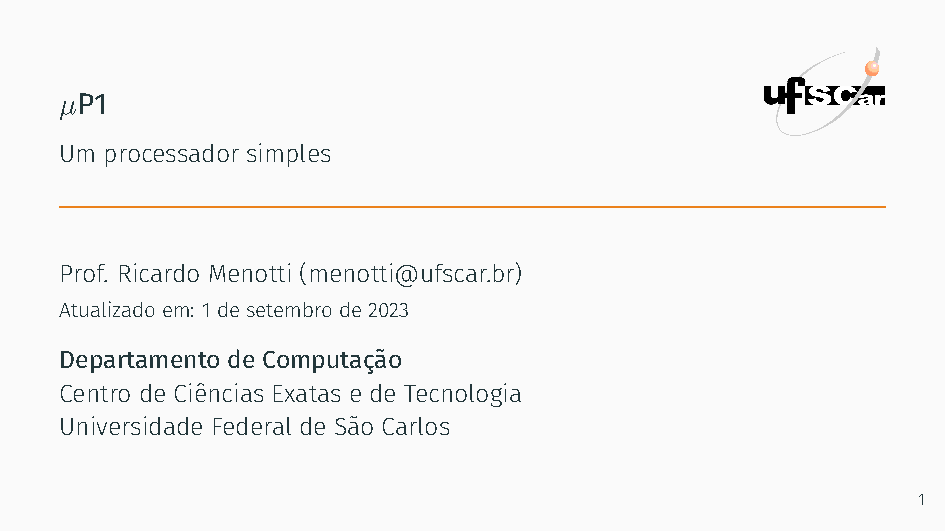
\includegraphics[width=\textwidth]{uP1}
            \href{https://www.edaplayground.com/x/sNSX}{Experimente ele aqui!}
        \end{column}
         \begin{column}{0.3\textwidth}
            \begin{verilogcode*}{firstnumber=0}
41  0100 0001  LOAD  A
52  0101 0010  ADD   B
33  0011 0011  STORE C
42  0100 0010  LOAD  B
31  0011 0001  STORE A
43  0100 0011  LOAD  C
32  0011 0010  STORE B
80  1000 0000  JUMP  0
            \end{verilogcode*}
            ... 
            \begin{verilogcode*}{firstnumber=240}
FF  1111 1111  // Dados            
00  0000 0000  // A
01  0000 0001  // B  
00  0000 0000  // C
            \end{verilogcode*}
        \end{column}
    \end{columns}
\end{frame}

\begin{frame}{Bibliografia}
    \small
\bibliographystyle{plainnat}
\bibliography{mm}
\end{frame}

\end{document}